\documentclass[12pt,a4paper]{article}

% ==== 导言区 ====
%================================
% note-setup-leftsidebox.tex
% fenglielie@qq.com 2025-09-12
%================================

\usepackage{amsmath,amsthm,amsfonts,amssymb}
\usepackage{mathtools}
\usepackage{mathrsfs}
\usepackage{bm}
\usepackage{extarrows}
\usepackage[a4paper, margin=1in]{geometry}
\usepackage{float}
\usepackage{indentfirst}
\usepackage{anyfontsize}
\usepackage{booktabs,multirow,multicol}
\usepackage[shortlabels,inline]{enumitem}
\usepackage{appendix}

\usepackage[dvipsnames]{xcolor}
\usepackage{graphicx}
\graphicspath{
    {./figure/}{./figures/}{./image/}{./images/}{./graphic/}{./graphics/}{./picture/}{./pictures/}
}
\usepackage{subcaption}
% TikZ-cd: commutative diagrams (loads tikz)
\usepackage{tikz-cd}
% Optional: enable additional tikz libraries if you need advanced arrow styles
\usetikzlibrary{arrows.meta,decorations.pathmorphing,cd}

\usepackage[ruled,linesnumbered,noline]{algorithm2e}
\usepackage{listings}
\lstdefinestyle{simpleStyle}{
    basicstyle=\ttfamily\small,
    breaklines=true,
    keywordstyle=\color{blue},
    identifierstyle=\color{black},
    stringstyle=\color{violet},
    commentstyle=\color[RGB]{34,139,34},
    showstringspaces=false,
    numbers=left,
    numbersep=2em,
    numberstyle=\footnotesize,
    frame=single,
    framesep=1em,
}
\lstset{style=simpleStyle}

\usepackage{hyperref}
\hypersetup{
    colorlinks=true,linkcolor=,urlcolor=cyan
}

\renewcommand*{\proofname}{\normalfont\bfseries Proof}

\usepackage{thmtools}

%% define environments
\declaretheorem[style=plain, name=Theorem, numbered=yes, numberwithin=section]{theoremplain}
\declaretheorem[style=plain, name=Proposition, numbered=yes, sibling=theoremplain]{propositionplain}
\declaretheorem[style=plain, name=Corollary, numbered=yes, sibling=theoremplain]{corollaryplain}
\declaretheorem[style=plain, name=Definition, numbered=yes, sibling=theoremplain]{definitionplain}


\declaretheorem[style=plain, name=Theorem, numbered=yes, numberwithin=section]{theorem}
\declaretheorem[style=plain, name=Theorem, numbered=no]{theorem*}

\declaretheorem[style=plain, name=Proposition, numbered=yes, sibling=theorem]{proposition}
\declaretheorem[style=plain, name=Proposition, numbered=no]{proposition*}

\declaretheorem[style=plain, name=Corollary, numbered=yes, sibling=theorem]{corollary}
\declaretheorem[style=plain, name=Corollary, numbered=no]{corollary*}

\declaretheorem[style=plain, name=Lemma, numbered=yes, sibling=theorem]{lemma}
\declaretheorem[style=plain, name=Lemma, numbered=no]{lemma*}

\declaretheorem[style=plain, name=Claim, numbered=yes, sibling=theorem]{claim}
\declaretheorem[style=plain, name=Claim, numbered=no]{claim*}

\declaretheorem[style=definition, name=Definition, numbered=yes, numberwithin=section]{definition}
\declaretheorem[style=definition, name=Definition, numbered=no]{definition*}

\declaretheorem[style=definition, name=Example, numbered=yes, numberwithin=section]{example}
\declaretheorem[style=definition, name=Example, numbered=no]{example*}

\declaretheorem[style=definition, name=Problem, numbered=yes, numberwithin=section]{problem}
\declaretheorem[style=definition, name=Problem, numbered=no]{problem*}

\declaretheorem[style=remark, name=Remark, numbered=yes, numberwithin=section]{remark}
\declaretheorem[style=remark, name=Remark, numbered=no]{remark*}

\declaretheorem[style=remark, name=Note, numbered=yes, numberwithin=section]{note}
\declaretheorem[style=remark, name=Note, numbered=no]{note*}

\declaretheoremstyle[headfont=\bfseries, bodyfont=\normalfont, spaceabove=3pt, spacebelow=3pt, qed=\ensuremath{\square}]{solutionstyle}

\declaretheorem[style=solutionstyle, name=Solution, numbered=yes, numberwithin=section]{solution}
\declaretheorem[style=solutionstyle, name=Solution, numbered=no]{solution*}

\usepackage[most]{tcolorbox}

\newcommand{\newtcbenvironment}[2]{
    \tcolorboxenvironment{#1}{#2, enhanced, breakable, sharp corners,leftrule=2pt, rightrule=0pt, toprule=0pt, bottomrule=0pt}
    \tcolorboxenvironment{#1*}{#2, enhanced, breakable, rounded corners,leftrule=2pt, rightrule=0pt, toprule=0pt, bottomrule=0pt}
}

%% define styles

\newtcbenvironment{theorem}{colframe=RoyalPurple, colback=RoyalPurple!8}
\newtcbenvironment{proposition}{colframe=RoyalPurple, colback=RoyalPurple!8}
\newtcbenvironment{corollary}{colframe=NavyBlue, colback=SkyBlue!8}
\newtcbenvironment{lemma}{colframe=NavyBlue, colback=SkyBlue!8}
\newtcbenvironment{claim}{colframe=NavyBlue, colback=SkyBlue!8}

\newtcbenvironment{definition}{colframe=ForestGreen, colback=ForestGreen!5}
\newtcbenvironment{example}{colframe=RawSienna, colback=RawSienna!5}
\newtcbenvironment{problem}{colframe=WildStrawberry!30, colback=WildStrawberry!5}

%% cbox
\newtcolorbox{cbox}[1][]{%
    enhanced,
    breakable,
    sharp corners,
    leftrule=2pt, rightrule=0pt, toprule=0pt, bottomrule=0pt,
    colframe=SkyBlue,
    colback=SkyBlue!8,
    #1
}

%% cover
\usepackage{titling}
\newcommand{\extrainfo}{}
\renewcommand{\extrainfo}[1]{\renewcommand{\extrainfocontent}{#1}}
\newcommand{\extrainfocontent}{}
\newcommand{\makecover}[1]{%
    \begin{titlepage}
    \newgeometry{margin=0in}
    \parindent=0pt
    \includegraphics[width=\linewidth]{#1} % size = 1280*1024
    \vfill
    \begin{center}
        \parbox{0.618\textwidth}{%
            \raggedleft{\bfseries \Huge \thetitle} \\[0.6pt]
            \rule{0.618\textwidth}{4pt} \\
        }
    \end{center}
    \vfill
    \begin{center}
        \parbox{0.618\textwidth}{%
          \raggedleft\Large
            \begin{tabular}{r}
                \theauthor \\
                \thedate \\
            \end{tabular}%
        }
    \end{center}
    \vfill
    \begin{center}
        \parbox[t]{0.7\textwidth}{\centering \itshape \extrainfocontent}
    \end{center}
    \vfill
    \end{titlepage}
    \restoregeometry
    \thispagestyle{empty}
}
% USAGE
% \extrainfo{xxx}
% \makecover{/path/to/cover.png}

%记号定义
\newcommand{\nn}{\mathbb{N}}
\newcommand{\zz}{\mathbb{Z}}
\newcommand{\qq}{\mathbb{Q}}
\newcommand{\rr}{\mathbb{R}}
\newcommand{\cc}{\mathbb{C}}
\newcommand{\ff}{\mathbb{F}}
\newcommand{\ffp}{\mathbb{F}_p}
\newcommand{\sph}{\mathbb{S}}
\newcommand{\Log}{\operatorname{Log}} % 调用你上传的 setup.tex 文件
% 或者你也可以直接把 setup.tex 的内容复制粘贴在这里

\title{\LaTeX{} Note Template}
\author{X}
\date{\today}

\extrainfo{Github: \href{https://github.com/Baudelaireee/Notebook}{https://github.com/Baudelaireee/Notebook}}
\begin{document}

% \maketitle
\makecover{cover/R.jpg}
\tableofcontents
\newpage 

\section{9/28 Notes for <<Calculus on Manifolds>> by Spivak}

\begin{problem*}
    Can we derive the explicit formula from an equation with several variables?
    Here are two examples :\\
    \begin{equation}
        x^2 + y^2 -1 =0
    \end{equation}
    and \begin{equation}
        e^{xy   } + \sin y + x^2 -2 =0
    \end{equation}
\end{problem*}

In the first example, it is clearly that we can express $y$ as a function of $x$ in a certain interval. But in the second example, it seems that we can draw a picture to visualize the implicit curve.

\begin{figure}[H]
    \centering
    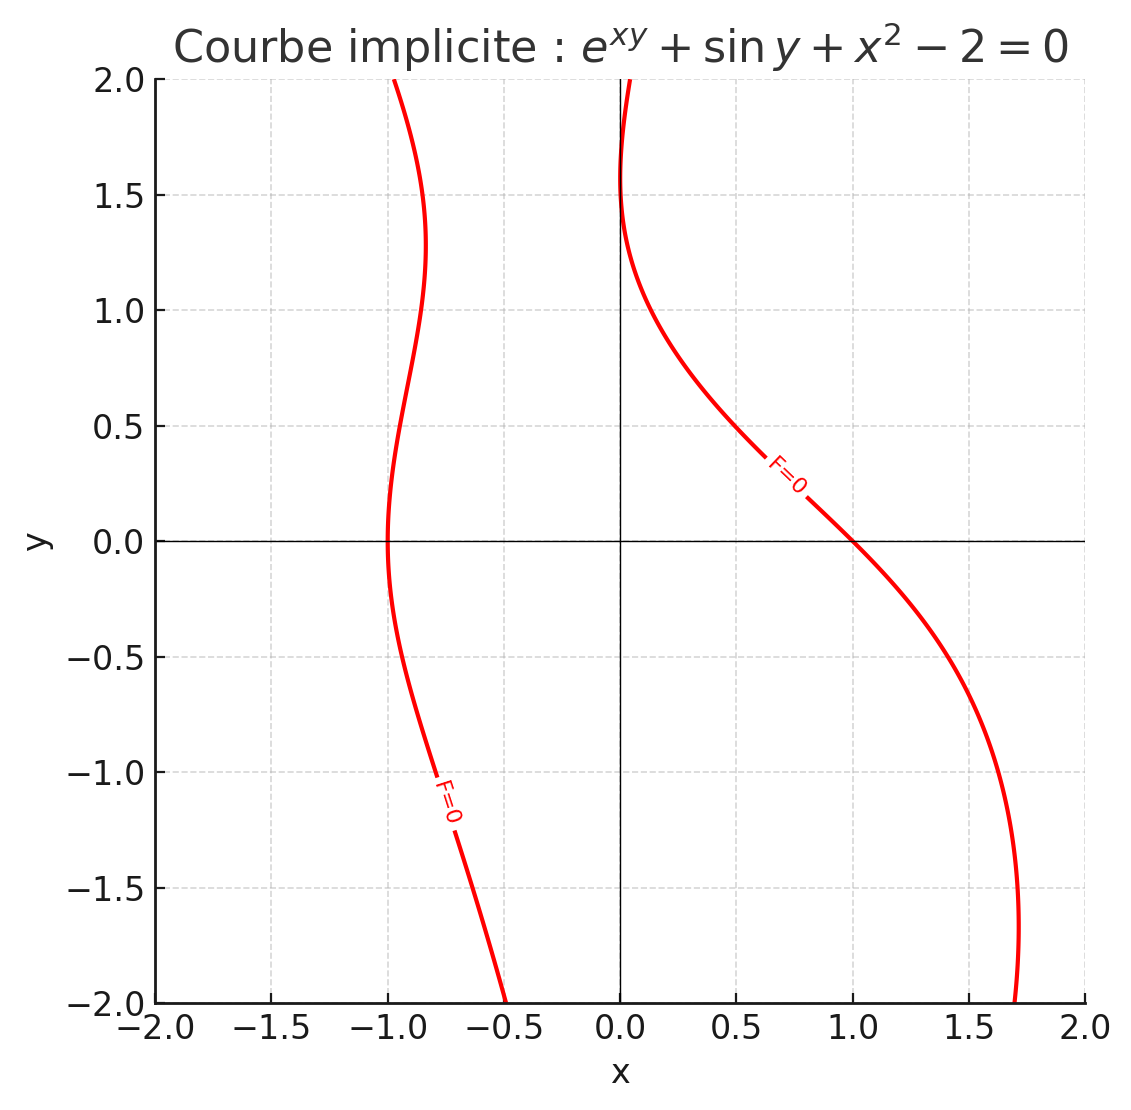
\includegraphics[width=0.7\textwidth]{implicit_curve.png}
    \caption{$e^{xy} + \sin y + x^2 - 2 = 0$}
    \label{fig:implicit_curve}
\end{figure}

The curve here seems very smooth, so for example, at the point \((x_0,0)\) in the curve we can express \(y\) as a function of \(x\) in the neighborhood, but it does not mean that we can write the function explicitly.

For thinking about this problem, we assume here we have a multivariable function \(F(x,y)\) and we want to solve the equation \(F(x,y)=0\). Like equation (1), we can express it as \(F(x,y) = x^2+y^2-1\). Here we assume \(F\) is a smooth function, then we can get the total differential of \(F\)
\[df = \frac{\partial F}{\partial x}dx + \frac{\partial F}{\partial y}dy\]
If we assume the existence of the implicit function \(y=f(x)\), then along the curve (\(G(x) = F(x,f(x)) = 0\)) we can get
\[0 = G'(x) =  \frac{\partial F}{\partial x}(x,f(x)) + \frac{\partial F}{\partial y}(x,f(x))\cdot f'(x) \]
hence we can get the derivative of the function \(f\) can be denoted by
\[f'(x) = -\frac{\frac{\partial F}{\partial x}(x,f(x))}{\frac{\partial F}{\partial y}(x,f(x))}\]
let us check some necessary condition here:\\
1. We try to restrict the function to be vanishing at some point, that means in the voisinage of the point, there exists something like a curve \(F(x,y)=0\) such that we can do the total differential like above, so here we need two conditions: locally, \(F(a,b) = 0\) for some point \((a,b)\) and a enough smooth function \(F\).\\
2. We need to make sure the formula for \(f'(x)\) makes sense, so locally \(\frac{\partial F}{\partial y}(a,b) \neq 0\).\\

Actually, under these hypotheses, we can prove the existence of the implicit function \(y= f(x)\) in the voisinage of the point \((a,b)\) such that \(F(x,f(x))=0\), which completes the implicit function theorem in the case of two variables.\\

\begin{theorem}[Implicit Function Theorem in \(\mathbb{R}^2\)]
Let \(F\) be a \(C^1\) function defined on an open set containing the point \((a,b)\). Assume that \(F(a,b) = 0\) and \(\frac{\partial F}{\partial y}(a,b) \neq 0\). Then there exists an open interval \(I\) containing \(a\), an open interval \(J\) containing \(b\), and a unique \(C^1\) function \(f: I \to J\) such that for all \(x \in I\), \(F(x, f(x)) = 0\). Moreover, the derivative of \(f\) is given by
\[f'(x) = -\frac{\frac{\partial F}{\partial x}(x,f(x))}{\frac{\partial F}{\partial y}(x,f(x))}\]
\end{theorem}

\begin{proof}
    here we just give a proof of the existence of the implicit function \(f\), the propoerties have benn proved as above. The idea here is to construct a locally diffeomorphism and then use the inverse function theorem.

    We take the map \(\Phi(x,y) = (x, F(x,y))\), then we can compute the Jacobian matrix of \(\Phi\) at the point \((a,b)\)
    \[D\Phi(x,y) = \begin{pmatrix}
        1 & 0 \\
        \frac{\partial F}{\partial x}(x,y) & \frac{\partial F}{\partial y}(x,y) 
\end{pmatrix}\]
The condition \(\frac{\partial F}{\partial y}(a,b) \neq 0\) implies \(\det D\Phi(a,b) \neq 0\) the Jacobian matrix is invertible, hence by the inverse function theorem, there exists an open set \(W\) containing \((a,b)\) and an open set \(W'\) containing \(\Phi(a,b) = (a,0)\) such that \(\Phi: W \to W'\) is a \(C^1\) diffeomorphism.

Finally we can construct the implicit function: the inverse \(\Phi^{-1}(x,y) = (x, g(x,y))\) for some \(C^1\) smooth function \(g\) in \(W'\), so we define the implicit function on the domain \(D = \{x \in \rr | (x,0) \in W'\}\) (\textbf{RMQ:} here D is the intersection of W' and the x-axis, notice that at least \((a,0) \in W'\), so \(D\) is not empty and can be seen as an open interval conatining \(a\))
\[f(x) = g(x,0)\]
then 
\[\Phi(x,f(x)) = \Phi(x,g(x,0)) = \Phi \circ \Phi^{-1}(x,0) = (x,0)\]
by the definition of \(\Phi\) we can conlude that \(F(x,f(x)) = 0\)
\end{proof}

Let us back to the two examples above, if we apply the implicit function theorem here, we can get a clear ODE for the implicit function \(y=f(x)\), that is an equivalent view of the implicit function theorem.
\begin{example}
    See the equation (2), we want to find the express of \(y\) as a function of \(x\), so see the whole equation as a curve \(F(x,y) = e^{xy} + \sin y + x^2 - 2\), then by the implicit function theorem, we can conclude a new realtionship between \(x\) and \(y\):
     \[y' = f'(x) = -\frac{F_x(x,y)}{F_y(x,y)} = -\frac{ye^{xy} + 2x}{xe^{xy} + \cos y}\]
    so finding the explicit formula of \(y\) is equivalent to solving above ODE to get a explicit solution. The information here is given by the differentail structure of the curve, and notice that the ODE conatins the original information about the curve.

    However, sometimes we can find the explicit formula of the implicit function, for example, in equation (1), we can express \(y\) as a function of \(x\) explicitly:
    \[y = \pm \sqrt{1-x^2}\]
    and the corresponding ODE here is \[y' = -\frac{x}{y}\]
    It's a separable ODE, we can solve it easily to get the explicit formula of the \(y=f(x)\).
    
\end{example}

\section{ CA: Some examples and technics}
\begin{example}
    We consider two algebraic number fields \(\qq(\sqrt{2})\) and \(\qq(\sqrt{5})\). and we can study the algebraic intger ring in two fields, then we can find that
    \[K = \qq(\sqrt{2}), \qquad \mathcal{O}_K  = \zz[\sqrt{2}]\]
    and 
    \[K = \qq(\sqrt{5}), \qquad \mathcal{O}_K  = \zz[\frac{1+\sqrt{5}}{2}]\]
    here \(X^2+X+1\) gives a monic polynomial with integer coefficients such that \(\frac{1+\sqrt{5}}{2}\) is a root, that shows that \(\frac{1+\sqrt{5}}{2}\) is an algebraic integer, so \(\zz[\sqrt{5}] \subsetneq \mathcal{O}_K\).
\end{example}

It's a classic example about ring of algebraic integers, we can say more about quadratic fields

\begin{theorem}
    Let \(d\) be an integer without square factors, and let \(K = \qq(\sqrt{d})\) be a quadratic field. Then the ring of integers \(\mathcal{O}_K\) is given by
    \[
    \mathcal{O}_K = 
    \begin{cases}
        \zz[\sqrt{d}] & \text{if } d \equiv 2, 3 \mod 4, \\
        \zz\left[\frac{1 + \sqrt{d}}{2}\right] & \text{if } d \equiv 1 \mod 4.
    \end{cases}
    \]
\end{theorem}

\begin{proof}
    One proof elementary is to use p-adic valuation, here is the outline:
    \begin{itemize}
        \item Prove the \textbf{main lemma}: \(a+b\sqrt{d}\) is an algebraic integer if and only if \(2a \in \zz\) and \(a^2 - db^2 \in \zz\).
        \item Verify that if \(a+b\sqrt{d}\) is an algebraic integer, then \(v_p(a)\geq 0\) and \(v_p(b) \geq 0\) for any odd prime \(p\). (Notice that here is not sufficent to say \(a,b \in \zz\))
        \item Consider the case of 2-adic valuation we can get the condition \(v_2(a) \geq -1\) and \(v_2(b) \geq -1\).
        \item Prove that \(v_2(a) = -1 \) and \(v_2(b) = -1\) if and only if \(d \equiv 1 \mod 4\), otherwise \(v_2(a) \geq 0\) and \(v_2(b) \geq 0\), then we can conclude the result.
    \end{itemize}
\end{proof}
Notice that it is not so easy to prove the similar result for cubic fields or higher degree fields, the concept of \textbf{integral basis} is useful here.\\

operatio of ideals: a useful techincs to compute the isomorphism.
\begin{proposition}
    Let \(M\) be a \(A\)-module, \(I\) be an ideal of \(A\) and \(N\) be a submodule of \(M\), then we have the isomorphism:
    \[I(M/N) \cong (IM+N)/N\]
    In particular, when \(M=A\) and \(N = J\) is a ideal, then we have
    \[I(A/J) \cong (I+J)/J\]
\end{proposition}
\begin{proof}
    we consider the natural map \(\pi: M \to M/N\). We can verify that \(I(M/N)\) is a submodule of \(M/N\), then by correspondence theorem, there exists a submodule in \(M\):
    \begin{align*}
    \pi^{-1}(I(M/N)) &= \pi^{-1}\{\sum_{\text{finite}}a_k\cdot(m_k+N) \mid a_k \in I, m_k \in M \}\\
    &= \pi^{-1}\{\sum_{\text{finite}} a_k m_k + N \mid a_k \in I, m_k \in M\} \\
    &= IM + N
    \end{align*}
    Then again by the image of natural map we can match
    \[I(M/N) = (IM+N)/N\]
\end{proof}

\begin{proposition}
    If \(I \subset R\) as a ideal, \(a \in I\) and \(b \notin I\), then 
    \[a+b \notin I\]
\end{proposition}
\begin{proof}
    If \(a+b \in I\), then \(b = (a+b) - a \in I\), which is a contradiction.
\end{proof}\

\newpage
\section{Infinite products}
The form of infinite products is important in complex analysis to study the poles and zeros of functions, here is the definition:

\begin{definition}
    Let \((a_n)_{n=1}^{\infty}\) be a sequence of complex numbers. The infinite product \(\prod_{n=1}^{\infty} a_n\) is said to converge if there exists \(N \in \nn\) such that:\\
    (1) \(a_n \neq 0\) for all \(n \geq N\)\\
    (2) the sequence of partial products\((\prod_{k=n}^N a_k)_{n \geq N}\) converges to a non-zero limit as \(n \to \infty\).\\
If the limit is zero, we say the product \textbf{diverges to zero}. If the limit does not exist, we say the product diverges.
\end{definition}
we avoid the case that some terms are zero, because it will make the product zero, which is not interesting; and we notice that if the sequence \((a_n)\) converges to zero, then the product will tend to zero trivally, so we need to avoid this case too. Anyway, the definition here is delicated enough to avoid any trival case.

\begin{proposition}[The properties of convergence]
    Let \((a_n)_{n=1}^{\infty}\) be a sequence of complex numbers such that the infinite product \(\prod_{n=1}^{\infty} a_n\) converges, then:\\
    (1) \(\lim_{n \to \infty} a_n = 1\)\\
    (2-LOG) If \(a_n \in \cc-\rr_{-}\) for sufficent large \(n\), then we have equivalent conidtion for the convergence of the product: the series \(\sum_{n=1}^{\infty} \Log a_n\) converges.\\
    (3-CVA) If \(\sum_{n \in \nn} |a_n| < \infty\), then the product \(\prod_{n=1}^{\infty} 1+a_n\) converges or diverges to zero.

    \begin{proof}
        (1) is immediate form \(a_n = (\prod_{k=1}^{n}a_k/\prod_{k=1}^{n-1}a_k)\) for \(n \geq 2\).\\
        (2) By the convergence of (1), for sufficent large \(n\), \(a_n\) stays near 1, hence we can choose the principal branch such that for sufficent large \(N\)
        \[\Log \prod_{n \geq N}a_n = \sum_{n \geq N} \Log a_n\]
        (3) If \(\sum_{n \in \nn} |a_n| < \infty\), so \(a_n\) converges to zero so we can expend 
        \begin{align*}
            \Log(1+a_n) = a_n-\frac{a_n^2}{2} + o(a_n^3)
        \end{align*}
        Then by (2), the series \(\sum_{n \in \nn} \Log(1+a_n)\) converges absolutely, hence the product converges or diverges to zero.
        
    \end{proof}
\end{proposition}

With the basic technics, we can study the products of fuctions, that's the core to construct some important functions like gamma function.
\begin{definitionplain}[Convergence of product of functions] $ \\$
    Let \((f_n)_{n \in \nn}\) be a sequence of continous function on a open set \(U\)\\
    - The product \(\prod_{n \in \nn} f_n\) converges pointwise to \(F\) on \(U\) if for each \(z \in U\), the product \(\prod_{n \in \nn} f_n(z)\) converges to \(F(z)\).\\
    - The product \(\prod_{n \in \nn} f_n\) converges uniformly to \(F\) on \(U\) if there exists \(N \in \nn\) such that for all \(n \geq N\), \(f_n\) does not vanish on \(U\) and the sequence of partial products \((\prod_{k=n}^N f_k)_{n \geq N}\) converges uniformly to \(F\) on \(U\).
\end{definitionplain}
Here is the definition following above definition, the zero of the functions in sequence may cause some problems, so there are some difficult in definition. Another clear definition is from \textbf{Henri Cartan's book}, here we give as a lemma:

\begin{lemma}
    In above definition, let \(K \subset U\) as a subset, then the product \(\prod_{n \in \nn} f_n\) converges uniformly on \(K\) if \(f_n\) satisfies the following condition:\\
    (1) \((f_n)_{n \in \nn}\) coverges uniformly to \(1\) on \(K\).\\
    (2) The series \(\sum_{n \in \nn}\Log f_n\) converges normally on \(K\).

    \begin{proof}
        By (1), for sufficent large \(N\), we have \(|f_N - 1| < 1/2\), so for all \(n \geq N\), \(\Log f_n\) is well defined and  \(f_n\) does not vanish on \(K\). so for any \(z \in K\)
        \[\Log \prod_{k=n}^N |f_k| = \sum_{k=n}^N |\Log f_k| \leq \sum_{k=n}^N \|\Log f_k\|_{K}\]
        it implies that the sequence of partial products converges uniformlly on \(K\) by weierstrass M-test. 
    \end{proof}
\end{lemma}

Infinite products is a strong tool to construct function with certain zeros, for example we can constryct a function with zeros at all integers like following:
\[z \prod_{n \geq 1} (1 - \frac{z^2}{n^2})\]
It is not difficult to verify that he product converges locally uniformlly to a holomorphic function, and one holomorphic function sharing the propoerties is \textbf{sine function}, actually we can prove that they are equally up to a constant factor, which is a famous result called \textbf{Euler's sine product formula}. With the following proposition, we can completely prove the formula:
\[\sin(\pi z) = \pi z \prod_{n \geq 1} (1 - \frac{z^2}{n^2})\]
The proof can be found in [Stein 2, page 142].
\begin{proposition}
    Let \((f_n)_{n \in \nn}\) be a sequence of holomorphic functions on an open set \(\Omega \subset \cc\), and suppose that the product \(\prod_{n \in \nn} f_n\) converges  \(\Omega\) to a function \(f\) locally uniformly, then\\
    (1) \(f\) is holomorphic on \(\Omega\)\\
    (2) The zeros and multiplicities of \(f\) follows from the sequence:
    \[Z(f) = \bigcup_{n \in \nn} Z(f_n) \qquad m_f(z)= \sum_{n \in \nn} m_{f_n}(z)\] 
    (3) If \(f_n\) does not vanish on \(\Omega\) for any \(n\), then the series of meromorphic functions \(\sum_{n \in \nn} f_n'/f_n\) converges locally uniformly on \(\Omega - Z(f)\) to \(f'/f\).
\end{proposition}
\begin{proof}
    It's the result of locally uniformlly convergence on the inifinite product, notice that the proof of (3) is referred to a idenetity:
    \[\frac{(\prod_{k=1}^nf_k)'}{\prod_{k=1}^nf_k} = \sum_{k=1}^n \frac{f_k'}{f_k}\]
    which can be proved by induction. Another point is that the proof of (2) needs that the multiplicities of zeros are finite, i.e. for any \(a \in \Omega\) we have
    \[\#\{n\in \nn | f_n(a) = 0\} < \infty\]
    Which is ensured by the definition of convergence of infinite product.
\end{proof}

There are two natural question arsing from Euler's formula, one is that if we find another entire function with zeros at all integers, whether the function is same with sine function up to coefficients or anything else? The other is that if there exists a general method to construct entire function with given finite or infinite zeros? The answer is from \textbf{Weierstrass's} construction.

Firstly, the zeros of holomorphic is isolated or discrete, so we the given zeros can not have any limit point in \(\cc\), hence the problem is limited to discrete set of points. \textbf{For finite zeros, we can use the fundamental theorem of algebra to construct a polynomial with given zeros}, so the problem is limited to infinite zeros. By Borel-Weierstrass theorem, we can deuduce that the set of zeros must be unbounded.

Another point about zero is that the multiplicity of zeros must be finite. Suppose that \(f\) is an non-zero entire function, then by propoerty of analytic function, \(f\) can be expended at any point \(z_0\) as a Taylor series
\[f(z) = \sum_{n=0}^{\infty} \frac{f^{(n)}(z_0)}{n!} (z - z_0)^n\]
If \(z_0 \) is a zero with inifinite multiplicity, then \(f^{(n)}(z_0) = 0\) for all \(n \in \nn\), hence \(f \equiv 0\) in the neighborhood of \(z_0\), which implies \(f \equiv 0\) in \(\cc\) by analytic countiuation, it is absurd. Together with the above statement, if \((a_n)_{n \in \nn}\) is the sequence of zeros, then the zeros must satisfy \(\lim_{n \to \infty} |a_n| = \infty\).

With the basic analysis of zeros, now we can consrtuct the entire function by given zeros. Notice that we can not simply combine the zeros together by linear terms
\[\prod_{n \in \nn} (z-a_n)\]
The product diverges for infinite unbounded zeros, so we can copy the idea of Euler's formula, i.e.
\[\prod_{n \in \nn} (1 - \frac{z}{a_n})\]
However, we can not ensure the convergence of the product, for example we take zeros as all positive integers. To ensure the convergence we need to add some extra terms in each factor, that is called \textbf{Weierstrass's canonical factors}.

\begin{lemma}
    We define the weierstrass's canonical factor of the degree \(p\) as
    \[E_p(z) := \begin{cases}
        (1-z) & p=0 \\
        (1-z)e^{(z + \frac{z^2}{2} + \cdots + \frac{z^p}{p})} & p \in \nn
    \end{cases}\]
    then the factor has the following propoerties:\\
    (1) It is an entire function with a simple zero at \(z=1\) and no other zeros.\\
    (2) It is a function of finite order \(p+1\).\\
    (3) For \(|z| \leq r <1\), we have the estimate
    \[|E_p(z)-1| \leq C_r|z|^{p+1}\]
    for some constant \(C_r > 0\). That means the larger the \(p\) is, the convergence of \(E_p(z)\) to 1 is faster.
\end{lemma}
\begin{proof}
    (1) and (2) is clear, we prove (3).
    \begin{align*}
        \log(E_p(z)) &= \log(1-z) + z + \frac{z^2}{2} + \cdots + \frac{z^p}{p}  \\
        &= -\sum_{n=1}^{\infty} \frac{z^n}{n} + (z + \frac{z^2}{2} + \cdots + \frac{z^p}{p}) \\
        &= -\sum_{n=p+1}^{\infty} \frac{z^n}{n} = O(|z|^{p+1})
    \end{align*}
    the expansion here is ensured by \(|z| < 1\), hence
    \[E_p(z) = \exp(\log E_p(z)) = 1 + O(|z|^{p+1})\]
    by expansion of expoential function \(e^z = 1+z+o(z^2)\), so we can conlude the result.
\end{proof}

So we can response the original question by collecting the above ideas:
\begin{theorem}[Weierstrass's Factorization Theorem] $ \\$
    Let \((a_n)_{n \in \nn}\) be a sequence of complex numbers such that \(\lim_{n \to \infty} |a_n| = \infty\), and we make convention that \(E_n(\frac{z}{0}):= z\), then the infinite product
    \[f(z) = \prod_{n=1}^{\infty} E_{n}(\frac{z}{a_n})\]
    converges locally uniformly in \(\cc\) to an entire function \(f\) whose zeros are precisely the points \(a_n\), with multiplicities by counting. Moreover, if \(g\) is any other entire function with the same zeros and multiplicities, then there exists an entire function \(h\) such that
    \[g(z) = f(z)e^{h(z)}\]
    for all \(z \in \cc\).
    
\end{theorem}

Another better theorem is given by \textbf{Hadamard}, it shows the growth of the entire function will influence the construction of the function by given zeros.
\begin{theorem}[Hadamard's Factorization Theorem] $ \\$
Suppose that \(f\) is an entire function of finite order \(\rho\) with zeros \((a_n)_{n \in \nn}\) (counting multiplicities), then there exists a polynomial \(P\) of degree at most \(k=\lfloor \rho \rfloor\) such that
\[f(z) = e^{P(z)}\prod_{n=1}^{\infty} E_{n}(\frac{z}{a_n})\]
\end{theorem}
\newpage

\section{Ideal}
Ideal is something like normal subgroups in group theory, it is important to reflect the structure and relationship of rings. Here is the definition:
\begin{definition}
    Let \(R\) be a commutative ring, a subset \(I \subset R\) is called a ideal of \(R\) if the following conditions are satisfied:\\
    (1) \(I\) is an additive subgroup of \(R\), that is for any \(a,b \in I\), we have \(a-b \in I\).\\
    (2) For any \(r \in R\) and any \(a \in I\), we have \(ra \in I\) and \(ar \in I\).
\end{definition}

\begin{remark}
    Here is something to add as the properties, proof is not diffcult:\\

    (1) Ideal \(I \subset R\) can be seen as an \(R\)-submodule of \(R\), roughly speaking, it can be seen as a "vector subspace". (The union of ideals is not necassary an ideal)\\

    (2) An ideal generated by a subset \(S \subset R\) is defined by 
    \[\langle S \rangle := \bigcap_{I \text{ ideal}, S \subset I} I\]
    it is the smallest ideal containing \(S\), and we can verify that
    \[\langle S \rangle = \{\sum_{\text{finite}} r_i s_i \mid r_i \in R, s_i \in S\}\]
    In particular, a \textbf{principal ideal} is an ideal of the form \((a) = \langle \{a\} \rangle\), i.e a ideal generated by a single element (or it is a cyclic \(R\)-module).\\

    (3) A useful statement: If a unit \(r \in I\), then \(I = R\).\\

    (4) The operation of ideal: \(IJ \subset I\cap J \subset I \subset \langle I\cup J \rangle\)
\end{remark}





\end{document}

